\section{外设和中断}

\subsection{概述}

\subsubsection{VGA像素映射的屏幕}

\begin{center}
    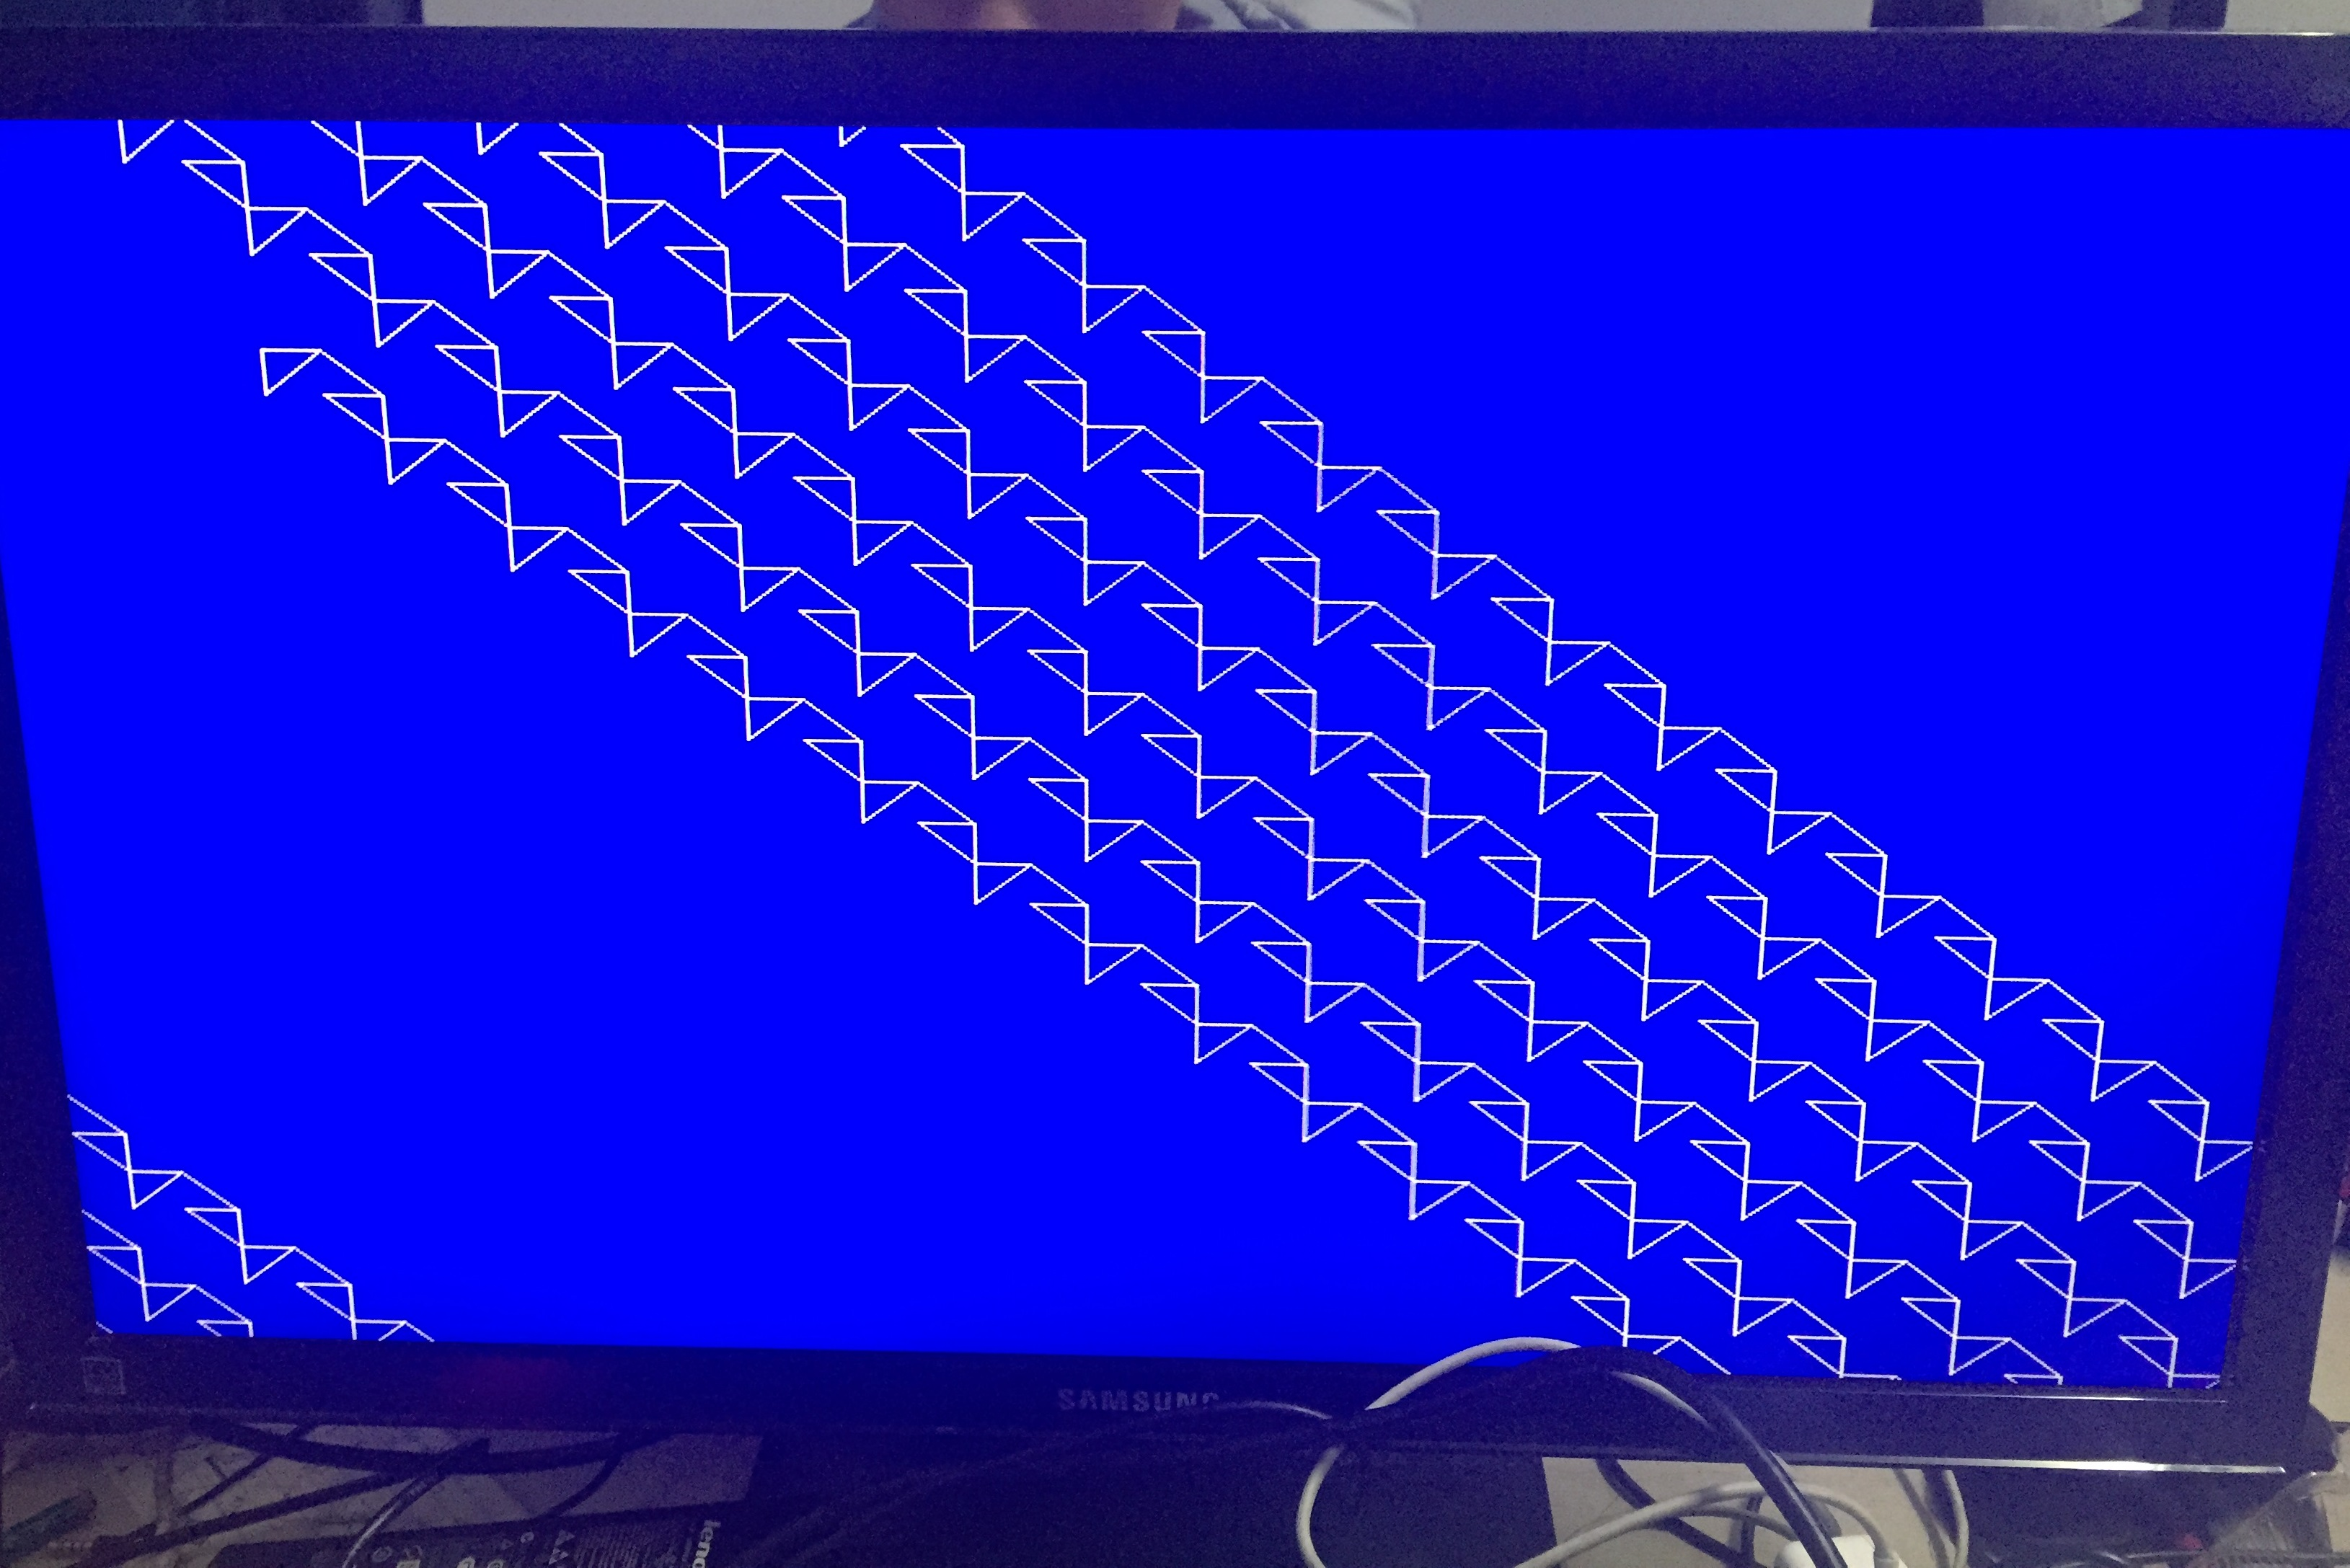
\includegraphics[height=10cm]{image/extension/tri.JPG}
    \fcaption{漂亮的三角形阵}\label{fig:tri}
\end{center}

屏幕为像素映射。我们在片内开了一块等同于屏幕可显示像素数目大小的RAM作为我们的显存(使用ISE的IP核)。我们只需修改显存即可改变屏幕上的内容,由于片内存储空间不大,所以只能显示蓝白两色。

像素映射为我们的计算机增添了\textbf{通用性}。

\subsubsection{键盘}

\begin{center}
    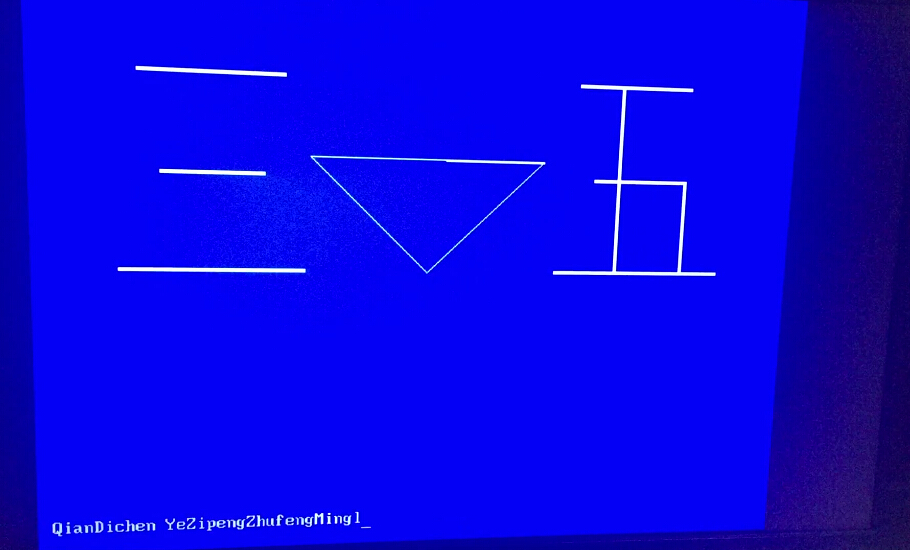
\includegraphics[height=10cm]{image/extension/35.JPG}
    \fcaption{软件中断和硬件中断的结合}\label{fig:35}
\end{center}

键盘拥有2个队列:一个叫做键盘队列,给硬件中断;一个叫做软中断队列,给软件中断。键盘输入一个字符,由硬件转译成ASCII码输送给键盘队列,当队列非空并且当时不在执行中断时,发送一个硬件中断信号,执行硬件中断。由硬件中断负责把信息转译到软中断队列。

\begin{enumerate}
    \item 实现0~9,a~z,退格键,空格键,回车键。硬件将其转化为ASCII码传入键盘队列
    \item 实现shift组合键,可以发送大写的字母,以及0~9上方的特殊字符
    \item 手写实现键盘队列(长度为8),软中断队列(长度为16)
\end{enumerate}


\subsubsection{硬件中断}

硬件中断是结合键盘和中央控制器实现的。每当键盘被按下,硬件中断被触发,我们会等待MEM,和WB段执行完,清空ID和ALU段。之后记录返回PC,改变PC到中断处理程序。


\subsection{细节}

\subsubsection{VGA像素映射的屏幕}

我们将大小为$640 \times 480$的整个屏幕映射到我们的显存上,我们用1位(0或1)来表示颜色,所以我们的显存空间总共为19位。 

我们的显存使用的是ISE自带的IP核,由于片内存储空间仅稍大于屏幕的可显示像素数目,我们只映射2种颜色。我们的RAM是读写端口分开的,由CPU进行写数据,由VGA控制器读出数据显示到屏幕上。

VGA控制器,我们使用了上学期老师发给我们的VGA扫屏代码,我们在其之上进行修改。由于我们的显存只够显示两种颜色(蓝色和白色),我们用0表示蓝色,1表示白色,扫屏的时候通过判断值来给RGB的线赋值。这样我们即可从我们的显存中读出屏幕的值。

CPU通过总线来写显存。由于16位的字长不足以表示整个屏幕,我们使用2个字(BF08和BF09)来向显存控制器写一个像素点,第一个字表示地址的高16位,第二个字包括地址的地位和写入的数据的RGB(这里的RGB仅仅是留作对软件的接口,由于我们只能显示2种颜色,所以我们只用1位)。

由于对于我们的这种表示来说,写一个模式(一个字母或者一个图形)对软件的要求极高,我们的工作有一部分也体现在软件上。这体现了我们的硬件的通用性,也考验我们硬件的鲁棒性。


\subsubsection{键盘,键盘队列以及软中断队列}

键盘的控制器是由上学期老师发的键盘代码修改而成的。

我们的键盘控制器能把通码转成ASCII码,滤去键盘不停发送的通码,直到接收到断码为止,也就是说我们的键盘不会导致失误。除此以外,我们支持组合键(shift + 按键可以产生大写的ASCII码),空格键,回车键,退格键······

键盘队列和软中断队列都是由我们自己实现。

这个队列是我们定义的一个模块,有2个端口,一个端口用于入队(写队列),一个端口用于出队(读队列)。每个端口都有各自的时钟(异步读写)和各自的使能端(如果不使能则队列保持不变)。队列内使用触发器存储数据,使用两个计数器来计数,分别表示队首和队尾。如果队首等于队尾则队列为空,否则队列非空,此时中断队列会发出中断信号,中央控制器会响应中断。

入队过程由上升沿触发,出队过程也是上升沿触发。是否入队/出队由入队/出队使能决定。键盘队列的容量是8个字,软中断队列的容量是16个字。

\subsubsection{硬中断}
我们每次按下键盘,键盘会将通码转换成ASCII码入队。这时队列的非空信号会触发一个硬件中断(由中央控制器实现)。

此时中央控制器会响应硬件中断,这是一个复杂的过程,整个流程分为如下几步:

\begin{enumerate}
    \item 锁住PC的写使能
    \item 存下EPC
    \item 清空流水线
    \item 跳转到中断处理程序
    \item 执行中断
    \item 中断返回
\end{enumerate}

我们详细说明如何清空流水线以及如何中断返回。

确定EPC:我们会先检查ID/ALU阶段寄存器的PC值是否为全0,如果不全0,我们将选择它。否则选择IF/ID段的PC值。为什么这样取呢?因为ID/ALU段可能是气泡,如果全0肯定是气泡,我们不能使用它。而我们整个流水线中不可能有连续2个气泡存在,所以选择IF/ID是安全的。

清空流水线:由于我们有分支预测,有插气泡的可能,我们认为流水线全部清空是不合适的。因为这时如果有分支预测错误,将不能复原。我们认为让流水线流完也是不合适的,此时PC的使能被锁住,如果有跳转将不能正常跳转。我们选择了一个折衷的方法,也是MIPS提倡的方法,把MEM和WB段的指令执行完,而ID和ALU段的指令清空。这样在我们的架构下不会产生冲突,中断得以正常进行。

中断返回:我们新增了一条ERET指令,代码是  FFFF  ,这条指令是中断执行程序的特权指令,只有在中断正在执行的时候才有效。这条指令会相当于一条B  EPC  ,表明中断执行结束,需要继续执行指令。

\subsubsection{软中断}
由软件实现,其过程需要等待硬中断的触发以及处理,通过硬中断把键盘队列中的数据转移到软中断队列中,软中断得以结束。

\section{软件方面}

\subsection{针对我们像素映射实现的接口}

\begin{enumerate}
    \item 给定坐标画一个点
    \item 给定起始点,长度,类型(总共8个类型,每45度角为一类)画一条细线段
    \item 给定起始点,长度,类型(同上),粗细,画一条粗线段
    \item 给定直角顶点,大小,类型(总共8个类型,每45度角为一类)画一个等腰直角三角形
    \item 从数据RAM中读取一个形状(用于实现字符集,比如汉字或是ASCII码)
\end{enumerate}




\subsection{针对键盘实现的硬件中断和软件中断的中断程序}

\subsubsection{硬件中断}

\begin{enumerate}
    \item 从键盘输入队列中取出一个ASCII码输出到串口
    \item 从键盘输入队列中取出一个ASCII码输入到软中断队列
    \item 从键盘输入队列中取出一个ASCII码,通过调用字符显示的函数显示到屏幕
    \item 实现退格键
\end{enumerate}

\subsubsection{软件中断}

(类似于scanf()  ,  支持char 和 int)
\begin{enumerate}
    \item 从软件中断队列中读取一个ASCII码
    \item 从软件中断队列中读取一串数字,直到空格,并解析成一个INT
    \item (暂未完成)完成一个画图程序,读入画图指令,解析成参数,传给画图函数实现画图的功能,由于时间紧张,汇编代码(1000+行)已经完成,然后没有调试完全,还不能工作。
\end{enumerate}

\subsection{定制的term}

\subsubsection{概述}
由于老师提供的term只支持基础指令,而我们需要调试也需要使用扩展的指令。

\begin{center}
    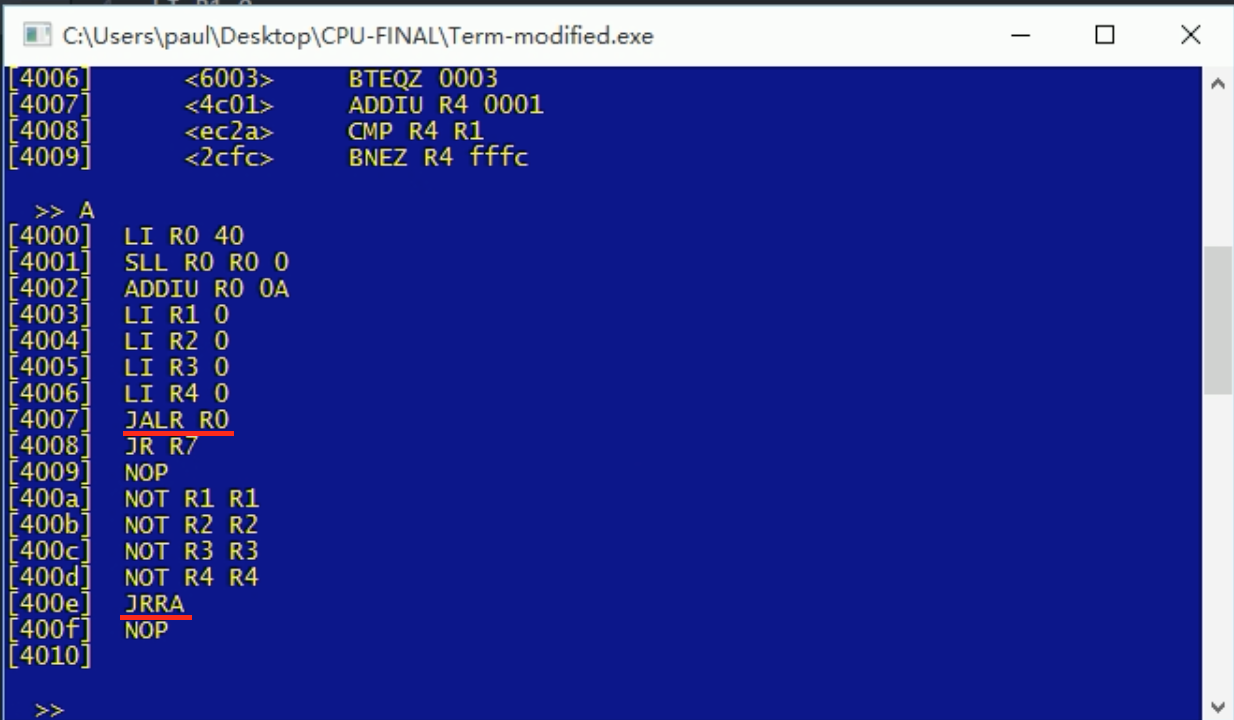
\includegraphics[height=10cm]{image/extension/term}
    \fcaption{扩展的Term}\label{fig:term}
\end{center}

\subsubsection{具体内容及实现}
我们自己的Term具备老师的Term的全部功能,除此以外,我们为它增添了新的特性,包括:
\begin{enumerate}
    \item 可以识别拓展的5条指令,包括NOT,BTNEZ,SLT,JALR,JRRA
    \item 可以向RAM中写入拓展的5条指令,包括NOT,BTNEZ,SLT,JALR,JRRA
    \item 中断的支持,对ERET的写入
\end{enumerate}

实现这个term的过程并不难,因为莱斯提供了term的源码,我们只需要在其A指令和U指令的模块中增加我们的指令即可。


